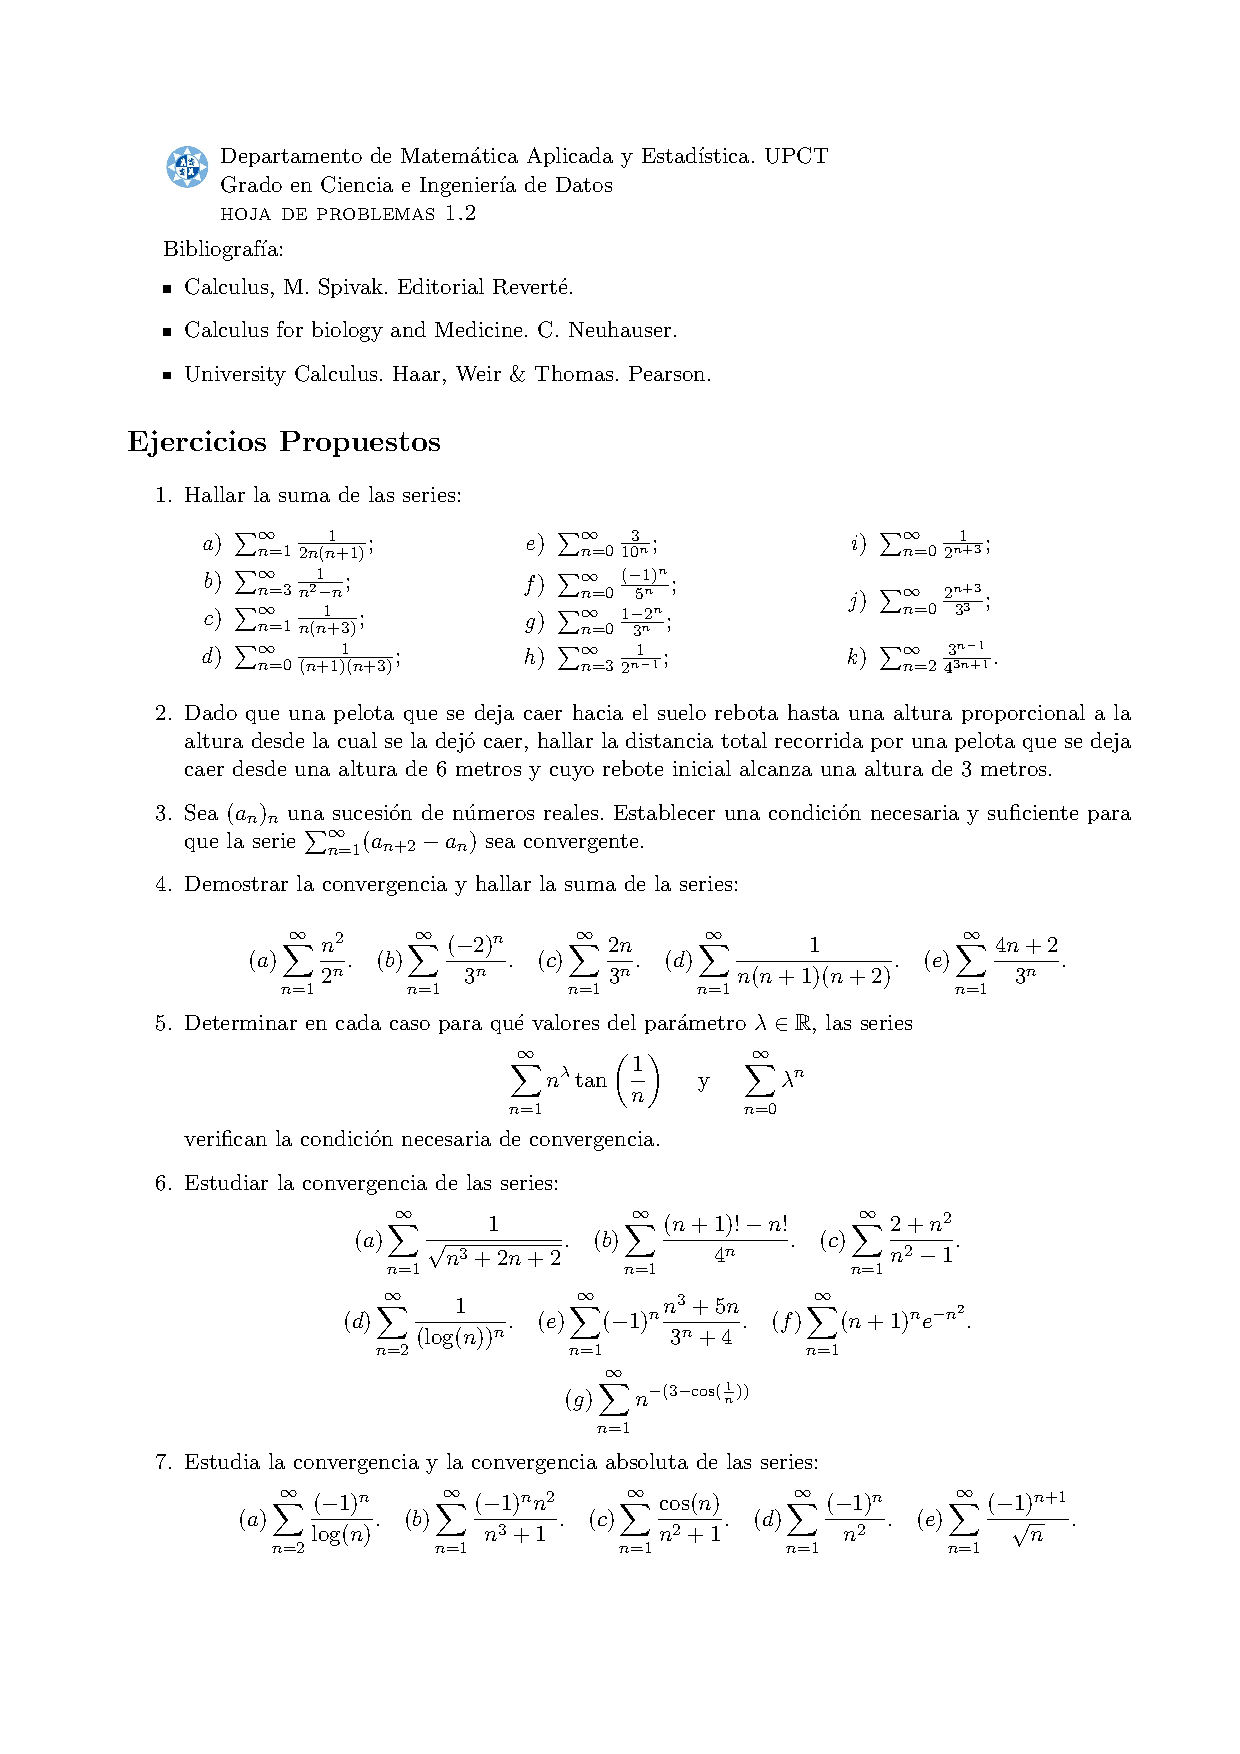
\includepdf[pages=-]{Tema 1/Hoja 1.2/Hoja 1.2.pdf}

\textcolor{red}{1) }\textcolor{lightblue}{Hallar la suma de las series:}

\begin{enumerate}[label=\color{red}\alph*)]
	\item $\textcolor{blue}{\sum_{n=1}^{\infty}\dfrac{1}{2n(n+1)}=}\lim_{n\to\infty}\mathcal{S}_m=\dfrac{1}{2}$
	
	$\begin{aligned}
		\mathcal{S}_m&=\sum_{n=1}^{m}\dfrac{1}{2n(n+1)}=\dfrac{1}{2\cdot1\cdot(1+1)}+\dfrac{1}{2\cdot2\cdot(2+1)}+\cdots+\dfrac{1}{2\cdot m\cdot(m+1)}\\
		&=\dfrac{1}{2}\sum_{n=1}^{m}\dfrac{1}{n}-\dfrac{1}{n+1}=\dfrac{1}{2}\left(\sum_{n=1}^{m}\dfrac{1}{n}-\sum_{n=2}^{m}\dfrac{1}{n+1}\right)=\dfrac{1}{2}\left(1+\cancel{\sum_{n=2}^{m}\dfrac{1}{n}}-\cancel{\sum_{n=2}^{m}\dfrac{1}{n}}-\dfrac{1}{m}\right)\\
		&=\dfrac{1}{2}\left(1-\dfrac{1}{m}\right)
	\end{aligned}$
	
	$\dfrac{1}{n(n+1)}=\dfrac{A}{n}+\dfrac{B}{n+1}=\dfrac{A\cdot(n+1)+B\cdot n}{n(n+1)}=\dfrac{(A+B)n+A}{n(n+1)}\longrightarrow (A+B)n+A=1\Rightarrow\left\{\begin{array}{l}
		A+B=0\\
		A=1
	\end{array}\right.$
	\item $\textcolor{blue}{\sum_{n=3}^{\infty}\dfrac{1}{n^2-n}=}\sum_{n=3}^{\infty}\dfrac{1}{n(n-1)}$
	
	$\mathcal{S}_m=\sum_{n=3}^{m}\dfrac{1}{n(n-1)}=\sum_{n=3}^{m}\dfrac{-1}{n}+\sum_{n=3}^{m}\dfrac{1}{n-1}=\textcolor{lightblue}{\underbracket[1pt]{\color{black}\sum_{n=3}^{m}-\dfrac{1}{n}+\dfrac{1}{n-1}}_{(\ast)}}=\sum_{n=3}^{m}\dfrac{1}{2}-\dfrac{1}{m}\xrightarrow[m\to+\infty]{}\bboxed{\dfrac{1}{2}}$
	
	$\dfrac{A}{n}+\dfrac{B}{n-1}=\dfrac{A(n-1)+Bn}{n(n-1)}=\dfrac{(A+B)n-A}{n(n-1)}\longrightarrow\left\{\begin{array}{l}
		A+B=0\\
		-A=1
	\end{array}\right.\qquad\boxed{\begin{array}{l}
		A=-1\\
		B=1
		\end{array}}$
	
	$\textcolor{lightblue}{(\ast)=}\left\{\begin{array}{r|c|l}
		\dfrac{1}{2} & \cancel{+\dfrac{1}{3}+\dfrac{1}{4}+\cdots+\dfrac{1}{n-1}} & \\
		 & \cancel{-\dfrac{1}{3}-\dfrac{1}{4}-\cdots-\dfrac{1}{m-1} }& -\dfrac{1}{m}
	\end{array}\right\}=\dfrac{1}{2}-\dfrac{1}{m}$
	\item $\textcolor{blue}{\sum_{n=1}^{\infty}\dfrac{1}{n(n+3)}=}\lim_{n\to\infty}\mathcal{S}_m$
	
	$\begin{aligned}
		\mathcal{S}_m&=\sum_{n=1}^{m}\dfrac{1}{n(n+3)}=\sum_{n=1}^{m}\dfrac{\frac{1}{3}}{n}+\dfrac{-\frac{1}{3}}{n+3}=\dfrac{1}{3}\left(\sum_{n=1}^{m}\dfrac{1}{n}-\sum_{n=1}^{m}\dfrac{1}{n+3}\right)=\dfrac{1}{3}\left(\sum_{n=1}^{m}\dfrac{1}{n}-\sum_{n=4}^{m+3}\dfrac{1}{n}\right)\\
		&=\dfrac{1}{3}\left(1+\dfrac{1}{2}+\dfrac{1}{3}+\cancel{\sum_{n=4}^{m}\dfrac{1}{n}}-\cancel{\sum_{n=4}^{m}\dfrac{1}{n}}-\dfrac{1}{m+1}-\dfrac{1}{m+2}-\dfrac{1}{m+3}\right)\\
		&=\dfrac{1}{3}\left(\dfrac{11}{6}-\dfrac{1}{m+1}-\dfrac{1}{m+2}-\dfrac{1}{m+3}\right)\xrightarrow[m\to+\infty]{}\dfrac{1}{3}\cdot\dfrac{11}{6}=\bboxed{\dfrac{11}{18}}
	\end{aligned}$
	
	$\dfrac{1}{n(n+3)}=\dfrac{A}{n}+\dfrac{B}{n+3}=\dfrac{A(n+3)+Bn}{n(n+3)}=\dfrac{(A+B)n+3A}{n(n+3)}\longrightarrow\left\{\begin{array}{l}
		A+B=0\\
		3A=1
	\end{array}\right.\qquad\boxed{\begin{array}{l}
			A=\dfrac{1}{3}\\
			B=-\dfrac{1}{3}
	\end{array}}$

	\item $\textcolor{blue}{\sum_{n=0}^{\infty}\dfrac{1}{(n+1)(n+3)}=}\lim_{n\to\infty}\mathcal{S}_m$
	
	$\begin{aligned}
		\mathcal{S}_m&=\sum_{n=0}^{m}\dfrac{1}{(n+1)(n+3)}=\sum_{n=0}^{m}\dfrac{\frac{1}{2}}{n+1}-\dfrac{\frac{1}{2}}{n+3}=\dfrac{1}{2}\textcolor{lightblue}{\underbracket[1pt]{\textcolor{black}{\left(\sum_{n=0}^{m}\dfrac{1}{n+1}-\dfrac{1}{n+3}\right)}}_{(\ast)}}\\
		&=\dfrac{1}{2}\left(1+\dfrac{1}{2}-\dfrac{1}{m+2}-\dfrac{1}{m+3}\right)\xrightarrow[m\to+\infty]{}\dfrac{1}{2}\left(1+\dfrac{1}{2}\right)=\dfrac{1}{2}\cdot\dfrac{3}{2}=\bboxed{\dfrac{3}{4}}
	\end{aligned}$
	
	$\dfrac{A}{n+1}+\dfrac{B}{n+3}=\dfrac{A(n+3)+B(n+1)}{(n+1)(n+3)}\longleftrightarrow1=A(n+3)+B(n+1)\longrightarrow\left\{\begin{array}{l}
		\text{Para }n=-1\longrightarrow A=\dfrac{1}{2}\\
		\text{Para }n=-3\longrightarrow B=-\dfrac{1}{2}
	\end{array}\right.$
	
	$\textcolor{lightblue}{(\ast)=}\left\{\begin{array}{r|c|l}
		1+\dfrac{1}{2} & \cancel{+\dfrac{1}{3}+\dfrac{1}{4}+\cdots+\dfrac{1}{m}+\dfrac{1}{m+1}} & \\
		& \cancel{-\dfrac{1}{3}-\dfrac{1}{4}-\cdots-\dfrac{1}{m}-\dfrac{1}{m+1}}&-\dfrac{1}{m+2}-\dfrac{1}{m+3}
	\end{array}\right\}=1+\dfrac{1}{2}-\dfrac{1}{m+2}-\dfrac{1}{m+3}$
	\item $\textcolor{blue}{\sum_{n=0}^{\infty}\dfrac{3}{10^n}=}3\sum_{n=0}^{m}\dfrac{1}{10^n}$
	
	$\begin{aligned}
		\mathcal{S}_m&=3\sum_{n=0}^{m}\dfrac{1}{10^n}=3\cdot\left(1+\dfrac{1}{10}+\dfrac{1}{10^2}+\cdots+\dfrac{1}{10^m}\right)\\
		&=3\left(\dfrac{1-\frac{1}{10^m}\cdot\frac{1}{10}}{1-\frac{1}{10}}\right)\xrightarrow[n\to+\infty]{}3\cdot\dfrac{1}{1-\frac{1}{10}}=3\cdot\dfrac{10}{9}=\bboxed{\dfrac{10}{3}}
	\end{aligned}$
	
	\item $\textcolor{blue}{\sum_{n=0}^{\infty}\dfrac{(-1)^n}{5^n}=}\sum_{n=0}^{\infty}\left(\dfrac{-1}{5}\right)^n$
	
	$\mathcal{S}_m=\sum_{n=0}^{m}\left(\dfrac{-1}{5}\right)^n=1-\dfrac{1}{5}+\dfrac{1}{5^2}-\dfrac{1}{5^3}+\cdots+\dfrac{(-1)^m}{5^m}=\dfrac{1-\frac{(-1)^m}{5^m}\cdot\left(\frac{-1}{5}\right)}{1-\left(\frac{-1}{5}\right)}\xrightarrow[n\to+\infty]{}\dfrac{1}{1+\frac{1}{5}}=\bboxed{\dfrac{5}{6}}$
	
	\item $\textcolor{blue}{\sum_{n=0}^{\infty}\dfrac{1-2^n}{3^n}=}$
	\item $\textcolor{blue}{\sum_{n=3}^{\infty}\dfrac{1}{2^{n-1}}=}\sum_{n=2}^{\infty}\dfrac{1}{2^n}$
	
	$\mathcal{S}_m=\sum_{n=2}^{m}\dfrac{1}{2^n}=\dfrac{1}{2^2}+\dfrac{1}{2^3}+\cdots+\dfrac{1}{2^m}=\dfrac{\frac{1}{2^2}-\frac{1}{2^m}\cdot\frac{1}{2}}{1-\frac{1}{2}}\xrightarrow[n\to+\infty]{}\dfrac{\frac{1}{4}}{\frac{1}{2}}=\bboxed{\dfrac{1}{2}}$
	\item $\textcolor{blue}{\sum_{n=0}^{\infty}\dfrac{1}{2^{n+3}}=}\sum_{n=3}^{\infty}\dfrac{1}{2^n}$
	\item $\textcolor{blue}{\sum_{n=0}^{\infty}\dfrac{2^{n+3}}{3^3}=}\sum_{n=0}^{+\infty}\dfrac{2^n\cdot2^3}{3^3}=\dfrac{8}{27}\sum_{n=0}^{+\infty}2^n$
    
    Pero como $\lim_{n\to\infty}2^n=+\infty\neq0\longrightarrow$ entonces no verifica la condición necesario que deben verificar las series de términos no negativos, y es que $\lim_{n\to\infty}a_n=0$.
   
   Por lo tanto, como no verifica la condición necesaria, entonces \underline{no} es convergente, es decir, las series es \lb{divergente} y su suma sería $+\infty$.
	
	\item $\textcolor{blue}{\sum_{n=2}^{\infty}\dfrac{3^{n-1}}{4^{3n+1}}=}\sum_{n=2}^{\infty}\dfrac{3^n\cdot3^{-1}}{(4^3)^n\cdot4}=\dfrac{1}{12}\sum_{n=2}^{\infty}\left(\dfrac{3}{4^3}\right)^n$
	
	
\end{enumerate}

\textcolor{red}{2) }\textcolor{lightblue}{Dado que una pelota que se deja caer hacia el suelo rebota hasta una altura proporcional a la altura desde la cual se la dejó caer, hallar la distancia total recorrida por una pelota que se deja caer desde una altura de 6 metros y cuyo rebote inicial alcanza una altura de 3 metros.}

$6+3+3+\dfrac{3}{2}+\dfrac{3}{4}+\cdots6+2\cdot 3$

\textcolor{red}{3) }\textcolor{lightblue}{Sea $(a_n)_n$ una sucesión de números reales. Establecer una condición necesaria y suficiente para que la serie $\sum_{n=1}^{\infty}(a_{n+2}-a_n)$ sea convergente.}

$a_n$ ¿Qué necesita para ser convergente?

$\sum_{n=1}^{}$

\textcolor{red}{4)} \textcolor{lightblue}{Demostrar la convergencia y hallar la suma de las series:}

\begin{enumerate}[label=\color{red}\alph*)]
	\item $\textcolor{blue}{\sum_{n=1}^{\infty}\dfrac{n^2}{2^n}}$
	
	$a_n=\dfrac{n^2}{2^n}$
	
	$\lim_{n\to\infty}a_n=\lim_{n\to\infty}\dfrac{\frac{(n+1)`2}{2^{n+1}}}{\frac{n^2}{2^n}}=\lim_{n\to\infty}\dfrac{(n+1=^2)}{2\cdot n^2}=\dfrac{1}{2}<1\longrightarrow$ convergente
	
	$\begin{array}{r}
		\mathcal{S}_m=\sum_{n=1}^{m}\dfrac{n^2}{2^n}\\
	\dfrac{1}{2}\sum_{n=1}^{m}\dfrac{n^2}{2^{n+1}}\\
	\hline
	\mathcal{S}_m-\dfrac{1}{2}=\dfrac{1}{2}\mathcal{S}_m=\sum_{n=1}^{m}\dfrac{n^2}{2^n}=\sum_{n=1}^{m}\dfrac{n^2}{2^{n+1}}
	\end{array}$
	
	$\begin{aligned}
		\dfrac{1}{2}\mathcal{S}_m & =\sum_{n=1}^{m}\dfrac{n^2}{2^n}-\dfrac{n=2}{m+1}\dfrac{(n-1)^2}{2^n}=\dfrac{1}{2}+\sum_{n=2}^{m}\dfrac{n^2}{2^n}-\sum_{n=2}^{m}\dfrac{(n-1)^2}{2^n}-\dfrac{m^2}{2^{m+1}}\\
		&=\dfrac{1}{2}+\sum_{n=2}^{m}\dfrac{n^2-(n-1)^2}{2^n}-\dfrac{m^2}{2^{m+1}}\\
		&=\dfrac{1}{2}-\dfrac{m^2}{2^{m+1}}+\sum_{n=2}^{m}\dfrac{2n-1}{2^n}
	\end{aligned}$
	
	$\dfrac{1}{2}\mathcal{S}_m=\dfrac{1}{4}-\dfrac{m^2}{2^{m+2}}+\sum_{n=2}^{m}\dfrac{2n-1}{2^{n+1}}$
	
	$\dfrac{1}{2}\mathcal{S}_m-\dfrac{1}{4}\mathcal{S}_m=\dfrac{1}{2}-\dfrac{m^2}{2^{m+1}}+\sum_{n=2}^{m}\dfrac{2n-1}{2^n}-\dfrac{1}{4}+\dfrac{m^2}{2^{m+2}}-\sum_{n=2}^{m}\dfrac{2n-1}{2^{n+1}}$
	
	$\begin{aligned}
		\dfrac{1}{4}\mathcal{S}_m&=\dfrac{1}{4}-\dfrac{m^2}{2^{m+1}}+\dfrac{m^2}{2^{m+2}}+\sum_{n=3}^{m+1}\dfrac{2(n-1)-1}{2^n}\\
		&=\dfrac{1}{4}-\dfrac{m^2}{2^{m+2}}+\dfrac{3}{4}+\sum_{n=3}^{m}\dfrac{2n-1}{2^n}-\sum_{n=3}^{m}\dfrac{2n-3}{2^n}-\dfrac{2m-1}{2^{m+1}}\\
		&=1-\dfrac{m^2}{2^{m+1}}+\dfrac{m^2}{2^{m+2}}-\dfrac{2m-1}{2^{m-1}}+\sum_{n=3}^{m}\dfrac{1}{2^{n-1}}
	\end{aligned}$
	
	$\begin{array}{l}
		\dfrac{1}{4}\mathcal{S}_m=1-\cancel{\dfrac{m^2}{2^{m+1}}}+\cancel{\dfrac{m^2}{2^{m+2}}}-\cancel{\dfrac{2m-1}{2^{m-1}}}+\dfrac{1}{2}-\cancel{\dfrac{1}{2^{m-1}}}\xrightarrow[m\to+\infty]{}1+\dfrac{1}{2}=\dfrac{3}{2}\\
		\dfrac{1}{4}\lim_{n\to\infty}\mathcal{S}_m=\dfrac{3}{2}\longrightarrow \lim_{n\to\infty}\mathcal{S}_m=\dfrac{4\cdot3}{2}=\bboxed{6}
	\end{array}$
	\item $\textcolor{blue}{}$
	\item $\textcolor{blue}{\sum_{n=1}^{\infty}\dfrac{2n}{3^n}}$
	
	$\lim_{n\to\infty}\dfrac{\frac{2(n+1)}{3^{n+1}}}{\frac{2n}{3^n}}=\lim_{n\to\infty}\dfrac{(n+1)}{3n}=\dfrac{1}{3}<1$
	
	Criterio del cociente $\longrightarrow$ convergente
	
	$\begin{array}{l}
		\mathcal{S}_m=\sum_{n=1}^{m}\dfrac{2n}{3^n}\\
		\dfrac{1}{3}\mathcal{S}_m=\sum_{n=1}^{m}\dfrac{2n}{3^{n+1}}\\ 	
		\end{array}$
		
		$\begin{aligned}
			\left(1-\dfrac{1}{3}\right)\mathcal{S}_m&=\sum_{n=1}^{m}\dfrac{2n}{3^n}-\sum_{n=1}^{m}\dfrac{2n}{3^{n+1}}=\sum_{n=1}^{m}\dfrac{2n}{3^n}-\sum_{n=2}^{m+1}\dfrac{2(n-1)}{3^n}\\
			\dfrac{2}{3}\mathcal{S}_m&=\dfrac{2}{3}+\sum_{n=2}^{m}\dfrac{2n}{3^n}-\sum_{m}^{n=2}\dfrac{2n-2}{2^n}-\dfrac{2m}{3^{m+1}}\\
			&=\dfrac{2}{3}+\sum_{n=2}^{m}\left(\dfrac{2n}{3^n}-\dfrac{2n-2}{3^n}\right)-\dfrac{2m}{3^{m+1}}\\
			&=\dfrac{2}{3}+2\cdot \boxed{\sum_{n=2}^{m}\dfrac{1}{3^n}}-\dfrac{2m}{3^{m+1}}\\
			&\xrightarrow[m\to+\infty]{}\dfrac{2}{3}+2\cdot\dfrac{3}{2}\cdot\left(\dfrac{1}{3^2}-\cancel{\dfrac{1}{3^{m-1}}}\right)-\cancel{\dfrac{2m}{3^{m+1}}}=\dfrac{2}{3}+\dfrac{1}{3}=\bboxed{1}
		\end{aligned}$
		
		\item $\textcolor{blue}{\sum_{n=1}^{\infty}\dfrac{1}{n(n+1)(n+2)}}$
		
		$\begin{aligned}
			\dfrac{1}{n(n+1)(n+2)}&=\dfrac{A}{n}+\dfrac{B}{n+1}+\dfrac{C}{n+2}\\
			&=\dfrac{A(n+1)(n+2)+Bn(n+2)+Cn(n+1)}{n(n+1)(n+2)}\\
			&1=A(n+1)(n+2)+Bn(n+2)+Cn(n+1)
		\end{aligned}$
		
		\begin{itemize}[leftmargin=*]
			\item Para $n=0\longrightarrow 1=2A\rightarrow A=\dfrac{1}{2}$
			\item Para $n=-1\longrightarrow 1=-B\rightarrow B=-1$
			\item Para $n=-2\longrightarrow1=2C\rightarrow C=\dfrac{1}{2}$
		\end{itemize}
		
		$\begin{aligned}
			\mathcal{S}_m&=\sum_{n=1}^{m}\dfrac{\frac{1}{2}}{n}-\sum_{n=1}^{m}\dfrac{1}{n+1}+\sum_{n=1}^{m}\dfrac{\frac{1}{2}}{n+2}=\dfrac{1}{2}\sum_{n=1}^{m}\dfrac{1}{n}-\dfrac{1}{2}\sum_{n=1}^{m}\dfrac{1}{n+1}-\dfrac{1}{2}\sum_{n=1}^{m}\dfrac{1}{n+1}+\dfrac{1}{2}\sum_{n=1}^{m}\dfrac{1}{n+2}\\
			&=\dfrac{1}{2}\left(\sum_{n=1}^{m}\dfrac{1}{n}-\sum_{n=2}^{m+1}\dfrac{1}{n}\right)-\dfrac{1}{2}\left(\sum_{n=1}^{m}\dfrac{1}{n+1}-\sum_{n=2}^{m+1}\dfrac{1}{n+1}\right)\\
			&=\dfrac{1}{2}\left(1+\cancel{\sum_{n=2}^{m}\dfrac{1}{n}}-\cancel{\sum_{n=2}^{m}\dfrac{1}{n}}-\dfrac{1}{m+1}\right)-\dfrac{1}{2}\left(\dfrac{1}{2}+\cancel{\sum_{n=2}^{m}\dfrac{1}{n+1}}-\cancel{\sum_{n=2}^{m}\dfrac{1}{n+1}}-\dfrac{1}{m+2}\right)\\
			&=\dfrac{1}{2}\left(1-\dfrac{1}{m+1}-\dfrac{1}{2}+\dfrac{1}{m+2}\right)\xrightarrow[m\to+\infty]{}\dfrac{1}{2}\cdot\left(1-\dfrac{1}{2}\right)=\dfrac{1}{2}\cdot\dfrac{1}{2}=\bboxed{\dfrac{1}{4}}
		\end{aligned}$
\end{enumerate}

\textcolor{red}{5)} \textcolor{lightblue}{Determinar en cada caso para qué valores del parámetro $\lambda\in\mathbb{R}$, las series \[ \sum_{n=1}^{\infty}n^\lambda\tan\left(\dfrac{1}{n}\right)\qquad\mathrm{y}\qquad\sum_{n=0}^{\infty}\lambda^n \] verifican la condición necesaria de convergencia.}

Condición necesaria de convergencia 

$\begin{array}{l}
	\sum_{n=1}^{\infty}n^\lambda\tan\left(\dfrac{1}{n}\right)\qquad\qquad\lambda<1\\
	\lim_{n\to\infty}n^\lambda\tan\left(\dfrac{1}{n}\right)=\lim_{n\to\infty}n^{\lambda-1}=0
\end{array}$

\textcolor{red}{6) }\textcolor{lightblue}{Estudiar la convergencia de las series:}
\begin{enumerate}[label=\color{red}\alph*)]
	\item $\textcolor{blue}{\sum_{n=1}^{\infty}\dfrac{1}{\sqrt{n^3+2n+2}}}$
	
	$\sum_{n=1}^{\infty}\dfrac{1}{n^{\frac{3}{2}}}$ convergente $\begin{array}{l}
		\lim_{n\to\infty}\dfrac{a_n}{b_n}=r\\
		\lim_{n\to\infty}\dfrac{\frac{n}{\sqrt{n^3+2n+2}}}{\frac{1}{n^{\frac{3}{2}}}}=1
	\end{array}$
	\item $\textcolor{blue}{\sum_{n=1}^{\infty}\dfrac{(n+1)!-n!}{4^n}=}\sum_{n=1}^{\infty}\dfrac{n!\cdot n}{4^n}$
	
	Criterio del cociente
	
	$\lim_{n\to\infty}\dfrac{\frac{(n+1)!(n+1)}{4^{n+1}}}{\frac{n!\cdot n}{4^n}}=\lim_{n\to\infty}\dfrac{(n+1)\cdot(n+1)}{4\cdot n}=\infty$
	\item $\textcolor{blue}{\sum_{n=1}^{\infty}\dfrac{2+n^2}{n^2-1}}$
	
	$\lim_{n\to\infty}\dfrac{2+n^2}{n^2-1}=1$ 
	
	No se cumple la condición necesaria de convergencia
	\item $\textcolor{blue}{\sum_{n=2}^{\infty}\dfrac{1}{(\log(n))^n}}$
	
	$\lim_{n\to\infty}\dfrac{\frac{1}{\log(n+1)^{n+1}}}{\frac{1}{\log(n)^n}}=\lim_{n\to\infty}\dfrac{\log(n)^n}{\log(n+1)^{n+1}}=\left\{\log(n+1)\equiv \log(n)\right\}=\lim_{n\to\infty}\dfrac{\cancel{\log(n)^n}}{\cancel{\log(n)^n}\cdot\log(n)}=0<1$
	\item $\textcolor{blue}{\sum_{n=1}^{\infty}(-1)^n\dfrac{n^3+5n}{3^n+4}}$
	\item $\textcolor{blue}{\sum_{n=1}^{\infty}(n+1)^n\mathrm{e}^{-n^2}}$
	\item $\textcolor{blue}{\sum_{n=1}^{\infty}n^{-\left(3-\cos\left(\frac{1}{n}\right)\right)}}$
\end{enumerate}

\textcolor{red}{7)} \textcolor{lightblue}{Estudia la convergencia y la convergencia absoluta de las series:}

\begin{enumerate}[label=\color{red}\alph*)]
	\item $\textcolor{blue}{\sum_{n=2}^{\infty}\dfrac{(-1)^n}{\log(n)}}$ convergente
	
	\begin{enumerate}[label=\arabic*), leftmargin=*]
			\item $\lim_{n\to\infty}\dfrac{1}{\log(n)}=0~{\color{green}\checkmark}$ (Absolutamente convergente)
			\item $a_n=\dfrac{1}{\log(n)}$ decreciente
	\end{enumerate}

$\lim_{n\to\infty}\dfrac{\frac{1}{\log(n)}}{\frac{1}{n}}=\lim_{n\to\infty}\dfrac{n}{\log(n)}=\lim_{n\to\infty}\dfrac{(n+1)-n}{\log(n+1)-\log(n)}=\lim_{n\to\infty}\dfrac{1}{\log\left(1+\frac{2}{n}\right)}=\lim_{n\to\infty}n=\infty$
	\item $\textcolor{blue}{\sum_{n=1}^{\infty}\dfrac{(-1)^nn^2}{n^3+1}}$
	

	\item $\textcolor{blue}{\sum_{n=1}^{\infty}\dfrac{\cos(n)}{n^2+1}}$
	$\sum\left|\dfrac{\cos(n)}{n^2+1}\right|\le\dfrac{1}{n^2+1}\qquad\sum_{n=1}^{\infty}\dfrac{1}{n^2+1}$ convergente
	
	$\sum_{n=1}^{\infty}\dfrac{1}{n^2}$
	\item $\textcolor{blue}{\sum_{n=1}^{\infty}\dfrac{(-1)^n}{n^2}}$ absolutamente convergente	
	\item $\textcolor{blue}{\sum_{n=1}^{\infty}\dfrac{(-1)^{n+1}}{\sqrt{n}}}\left\lbrace\begin{array}{l}
		\mathrm{convergente}\\
		\sum_{n=1}^{\infty}\dfrac{1}{n^{\sqrt{2}}} \text{ divergente}
	\end{array}\right.$
	
	\begin{tikzpicture}% function
		\begin{axis}[xlabel=x,ylabel=y, axis lines=center]
			\addplot[lightblue, samples=150, domain=-1:2] {x^2};
			\addplot[blue, samples=150, domain=-1:1.7] {x^3};
		\end{axis}
	\end{tikzpicture}
\end{enumerate}

